\documentclass[10pt]{article}
\usepackage[utf8]{inputenc}

\usepackage[backend=bibtex,
style=numeric,
bibencoding=ascii
]{biblatex}
\usepackage{authblk}
\usepackage{graphicx}
\usepackage[bottom]{footmisc}
\usepackage{listings}
\usepackage{geometry}
\usepackage{enumitem}

\geometry{
  paperheight=8.5in,
  paperwidth=5.5in,
  left=10mm,
  top=20mm,
}

\addbibresource{sample.bib}

\title{Manuscript Formatting Instructions
\footnote{
Copyright \copyright 2018 by the Consortium for Computing Sciences in Colleges. Permission to copy without fee all or part of this material is granted provided that the copies are not made or distributed for direct commercial advantage, the CCSC copyright notice and the title of the publication and its date appear, and notice is given that copying is by permission of the Consortium for Computing Sciences in Colleges. To copy otherwise, or to republish, requires a fee and/or specific permission.}}
%\date{}
\date{\vspace{-7ex}}

\author[1]{Baochuan Lu}
\author[1]{Author A}
\author[2]{John Meinke}
\author[2]{Author B}

\affil[1]{\footnotesize
Computer and Information Sciences \protect\\
Southwest Baptist University \protect\\
Bolivar, MO 65613}
\affil[ ]{\textit {\{blue,auther\}@sbuniv.edu}}

\affil[2]{\footnotesize
Computer Science Department \protect\\
Excellent University \protect\\ Our Town, TX 00000}
\affil[ ]{\textit {\{email1,email2,email3,email4,email5\}@xyz.edu}}


\begin{document}


\maketitle

\begin{abstract}
This document describes manuscript formatting requirment for CCSC conferences. Authors can use this document as a template to format their papers.
\end{abstract}

\section*{Length}
Prepare the paper for written understanding with length approximately six (6) single spaced pages including tables, figures, and a list of references or bibliography.

\section*{Style}
Write clearly and simply in the third person for an audience that is well-grounded in computing, but who may have limited exposure or knowledge about the specific topic of your paper. Define any technical terms deemed to require clarification when they are introduced.

\section*{Title and Author Information}
Please follow the example in this paper to typeset title and author information.

\section*{Body of the Manuscript}
The text may be organized into sections and subsections. Please use \verb+\section+ and  \verb+\subsection+ commands to define them as show in this example paper. Latex will take care of the formatting. If you opt to number your sections and subsections, do so specifically using Arabic numbers.

\subsection*{1 Abstract}
Provide a one paragraph brief overview of the paper in both the manuscript for review and in the final manuscript for publication.

\subsection*{2 Citation}
Appropriately cite all references to other published works included in the paper. \texttt{biblatex} is used to create a list of references or bibliography as the last section in the paper. Here are citation examples for a book\cite{latexcompanion}, a jouranl paper\cite{einstein}, a website\cite{knuthwebsite}, and a conference proceeding paper\cite{maurer}.

\subsection*{3 Lists}
Lists are easy to create in  \LaTeX\ whether they are ordered, unordered, or nested as shown in the following exmaple.

\begin{itemize}[noitemsep]
  \item The individual entries are indicated with a black dot, a so-called bullet.
  \item The text in the entries may be of any length.
\end{itemize}

\begin{enumerate}[noitemsep]
  \item The labels consists of sequential numbers.
  \item The numbers starts at 1 with every call to the enumerate environment.
\end{enumerate}

\begin{enumerate}[noitemsep]
   \item The labels consists of sequential numbers.
   \begin{itemize}[noitemsep]
     \item The individual entries are indicated with a black dot, a so-called bullet.
     \item The text in the entries may be of any length.
   \end{itemize}
   \item The numbers starts at 1 with every call to the enumerate environment.
\end{enumerate}

\subsection*{4 Math Expressions}
The mass-energy equivalence is described by the famous equation

$$E=mc^2$$

discovered in 1905 by Albert Einstein.
In natural units ($c$ = 1), the formula expresses the identity

\begin{equation}
E=m
\end{equation}

\subsection*{5 Tables and Figures}
Include all tables and figures within the body of the text. (Provide as separate files in the original format any figures so that if there are problems with the figures coming into the final manuscript there are alternatives available to the editors.)

Here is an example Table \ref{table:nonlin}.

\begin{table}[ht]
\caption{Nonlinear Model Results} % title of Table
\label{table:nonlin} % is used to refer this table in the text
\centering % used for centering table
\begin{tabular}{c c c c} % centered columns (4 columns)
\hline\hline %inserts double horizontal lines
Case & Method\#1 & Method\#2 & Method\#3 \\ [0.5ex] % inserts table
%heading
\hline % inserts single horizontal line
1 & 50 & 837 & 970 \\ % inserting body of the table
2 & 47 & 877 & 230 \\
3 & 31 & 25 & 415 \\
4 & 35 & 144 & 2356 \\
5 & 45 & 300 & 556 \\ [1ex] % [1ex] adds vertical space
\hline %inserts single line
\end{tabular}
\end{table}

Here is an example Figure \ref{figure:universe}.

\begin{figure}[h!]
\centering
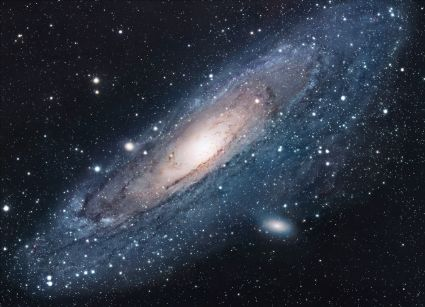
\includegraphics[scale=1.7]{universe}
\caption{The Universe}
\label{figure:universe}
\end{figure}

\subsection*{6 Reference List}
The \verb+\printbibliography+ command prints a list of referneces for you. Please use \texttt{sample.bib} as an example to create your bibliography entries.

\subsection*{7 Code Listings}
Commands from \texttt{listings} package allows you to display code easily and coloring and styling can be customized too. Here is an example.

\begin{lstlisting}[language=Python,  caption=Python example]
x = 42
epsilon = 0.01
step = epsilon**2
num_guesses = 0
ans = 0.0
while abs(ans**2-x) > epsilon and ans < x:
    ans = ans + step
    num_guesses += 1
if abs(ans**2-x) <= epsilon:
    print(str(ans) +
    ' is close to the square root of ' +
    str(x))
else:
    print('Failed to find square root of ' + str(x))
print("The number of guesses is " + str(num_guesses))
\end{lstlisting}

\section*{Additional Information}
Please feel free to email \verb+ccsc-editors@googlegroups.com+ for questions.

\medskip

\printbibliography

\end{document}
